%!TEX root = paper.tex

\section{Computational Results}\label{sec:comp}

We compare the training and test set accuracy for all of the simulated datasets, which are summarized in Table~\ref{tab:all_acc}.
The predictive function for standard logistic regression is simple and the predictive function for MFVB logistic regression has already been discussed in Section~\ref{sec:implement}.  However, the predictive function for MCMC is new, and we will describe here our method.  To predict the label $P(y=1|\M{x})$ for MCMC, we use the predictive function for MFVB logistic regression, except substituting the empirical mean $\M{\bar x}$ and empirical covariance ${\hat \Sigma}$ from the MCMC samples in place of the MFVB mean $\M{w}_N$ and standard deviation $\M{V}_N$.
 
Overall, we see that MCMC yields the highest out-of-sample accuracy in all cases except for Dataset 9.  (In Dataset 7, no result for
MCMC was reported because the data was separable.)  Logistic Regression is the second strongest method, and for most datasets logistic regression yields out-of-sample accuracy results matching MCMC.  Here, MFVB performs worse than the other methods, which is expected because MFVB requires the most restrictive set of assumptions: namely that the joint distribution factorizes into independent marginals.  Because MFVB is an approximate method, it much runs faster than MCMC, but as a result may sacrifice some predictive power.  For larger problems with many observations $n$ and high-dimension $p$, this tradeoff between computational complexity and performance may become more severe.  


\begin{table}[tb]
\centering
\begin{tabular}{rcccccc}
  \toprule
 {\bf  Dataset} & {\bf  Logit Train} & {\bf  Logit Test} & {\bf  MCMC Train} & {\bf  MCMC Test} & {\bf  MFVB Train} & {\bf  MFVB Test}\\
  \midrule
  0 & 0.8700 & {\bf 0.8580} & 0.8700 & {\bf 0.8580} & 0.8600 & 0.8570 \\
  1 & 0.7500 & 0.8450 & 0.7500 & {\bf 0.8460} & 0.7400 & 0.8450 \\
  2 & 0.5500 & {\bf 0.4890} & 0.5100 & {\bf 0.4890} & 0.5400 & 0.4750 \\
  3 & 0.6900 & {\bf 0.7420} & 0.6900 & {\bf 0.7420} & 0.7200 & 0.7120 \\
  4 & 0.8600 & {\bf 0.8050} & 0.8600 & {\bf 0.8050} & 0.8600 & 0.8040 \\
  5 & 0.9400 & 0.9290 & 0.9400 & {\bf 0.9300} & 0.9400 & 0.9260 \\
  6 & 0.7400 & 0.7130 & 0.7400 & {\bf 0.7140} & 0.6900 & 0.6840 \\
  7 & 1.0000 & 0.9760 & 1.0000 & *** & 1.0000 & {\bf 0.9780} \\
  8 & 0.9200 & {\bf 0.8670} & 0.9200 & {\bf 0.8670} & 0.9300 & 0.8640 \\
  9 & 0.5200 & 0.3980 & 0.5100 & 0.4020 & 0.4600 & {\bf 0.4130} \\
  10 & 0.6700 & 0.6690 & 0.6700 & {\bf 0.6700} & 0.6300 & 0.6560 \\
  \bottomrule
\end{tabular}
\caption{Training and test set accuracy for logistic regression, MCMC logistic regression, and MFVB logistic regression on all datasets.  The highest out-of-sample accuracy score is highlighted for each dataset.  \\ *** : The training dataset was completely separable; therefore the posterior covariance matrix was zero and the precision matrix was undefined.  Thus, we did not obtain MCMC predictive probabilities for this dataset. }\label{tab:all_acc}
\end{table}


\begin{figure}[h!]
\centering
    \begin{subfigure}[b]{0.45\textwidth}
	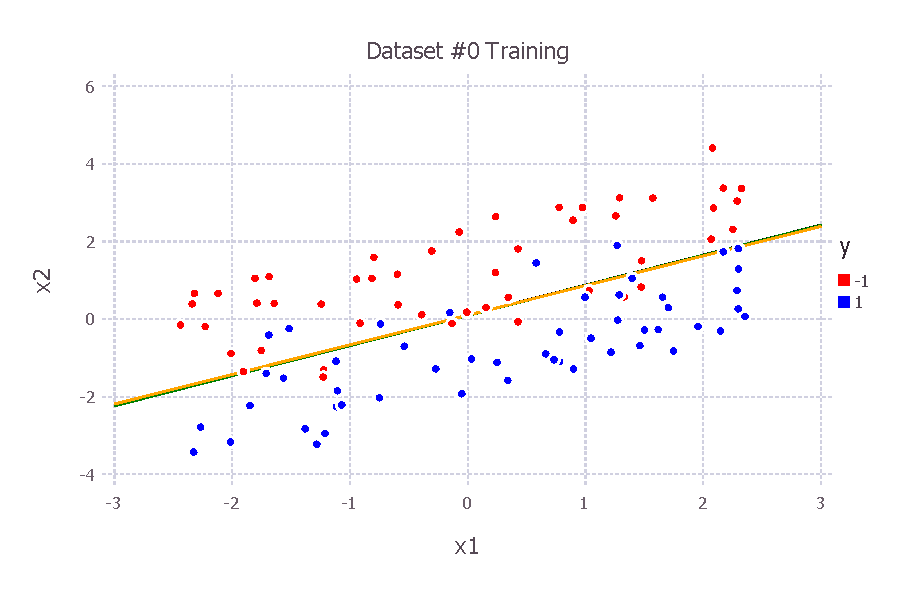
\includegraphics[scale=0.6]{figures/train_final_0.pdf}
    \end{subfigure}
    \quad
    \begin{subfigure}[b]{0.45\textwidth}
	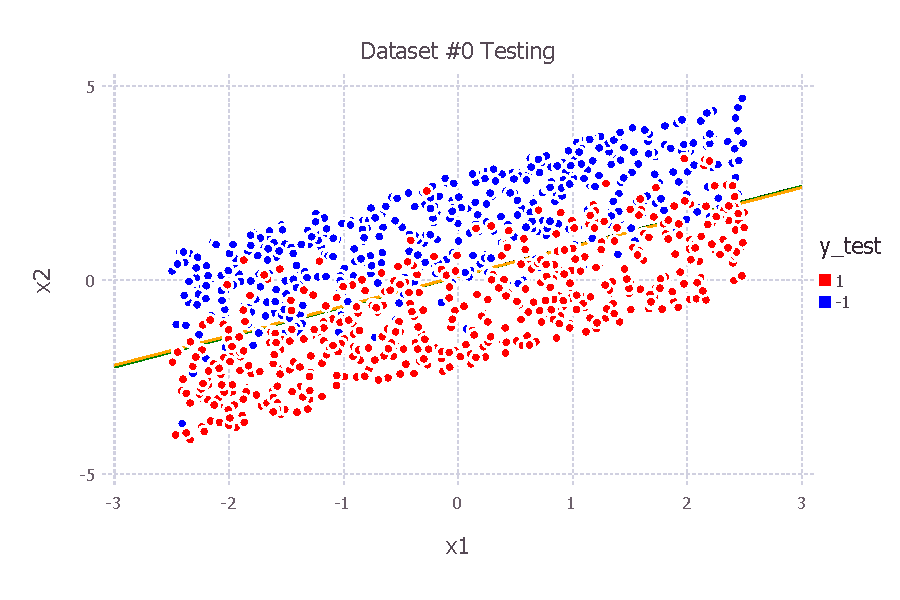
\includegraphics[scale=0.6]{figures/test_final_0.pdf}
	\end{subfigure}
    \caption{Plots of decision boundaries from Dataset 0.}  \label{fig:dataset_0}  
\end{figure}
\begin{figure}[h!]
\centering
    \begin{subfigure}[b]{0.45\textwidth}
	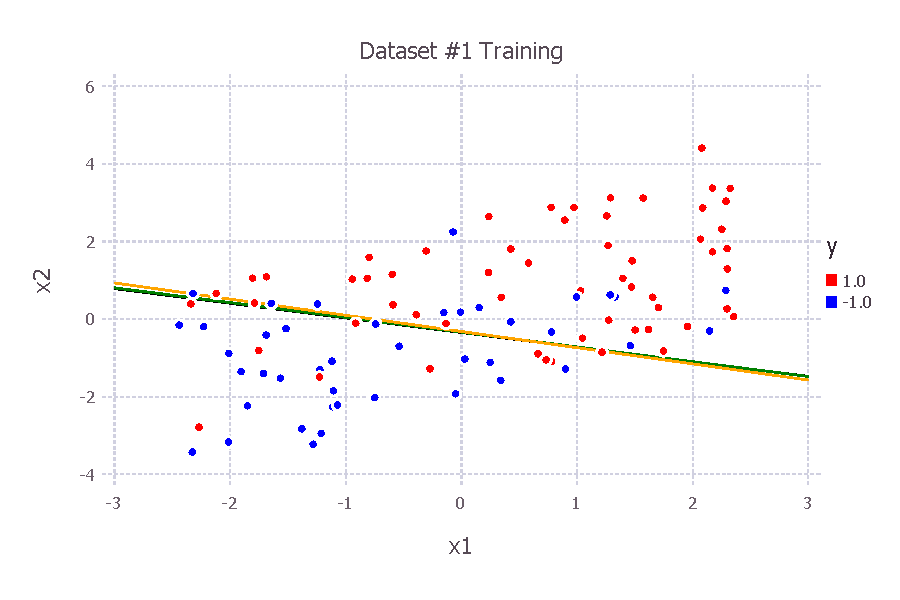
\includegraphics[scale=0.6]{figures/train_final_1.pdf}
    \end{subfigure}
    \quad
    \begin{subfigure}[b]{0.45\textwidth}
	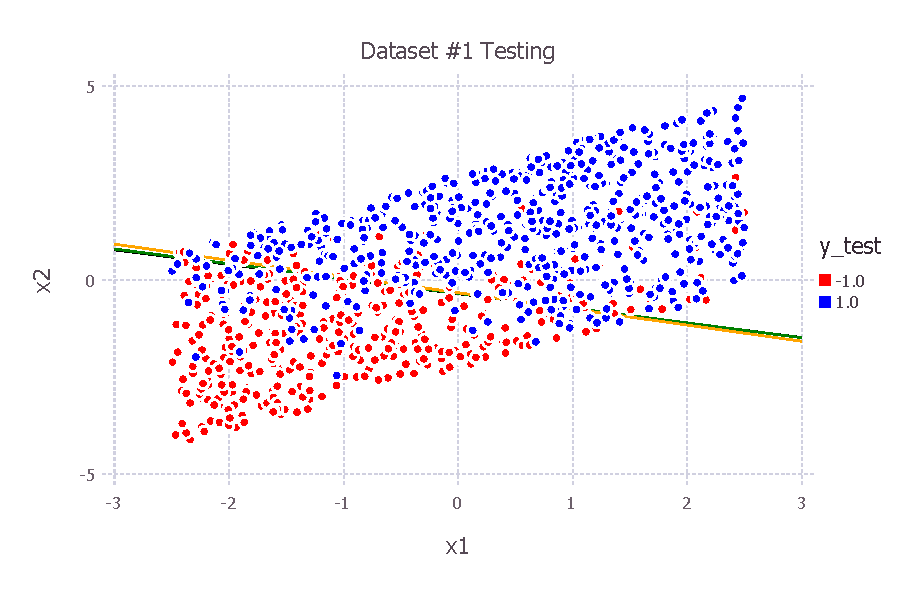
\includegraphics[scale=0.6]{figures/test_final_1.pdf}
	\end{subfigure}
    \caption{Plots of decision boundaries from Dataset 1.}  \label{fig:dataset_1}  
\end{figure}
\begin{figure}[h!]
\centering
    \begin{subfigure}[b]{0.45\textwidth}
	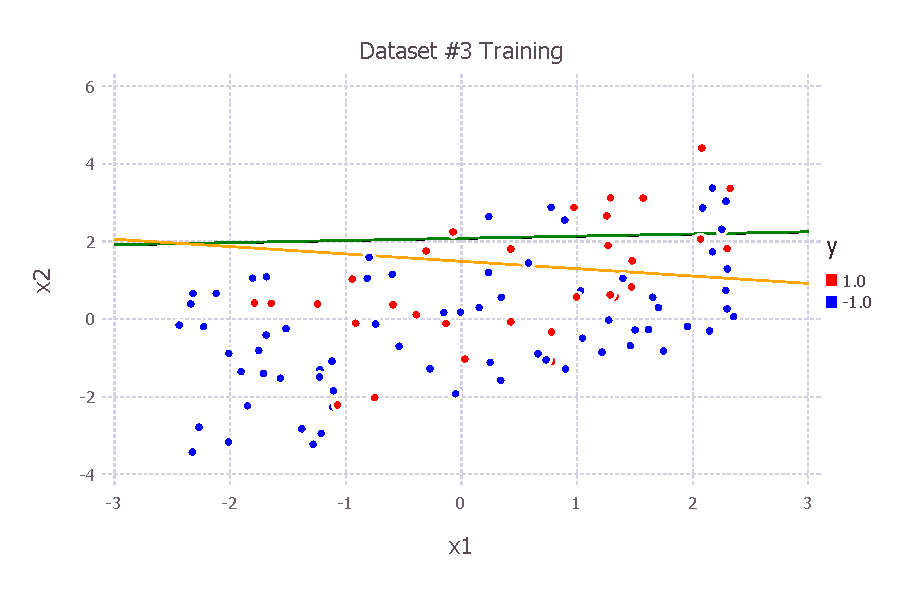
\includegraphics[scale=0.6]{figures/train_final_3.pdf}
    \end{subfigure}
    \quad
    \begin{subfigure}[b]{0.45\textwidth}
	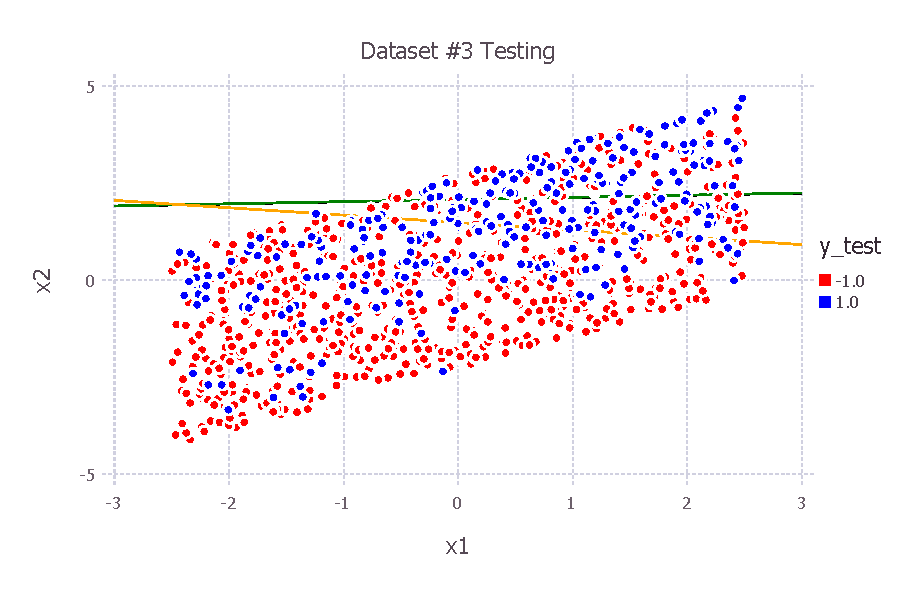
\includegraphics[scale=0.6]{figures/test_final_3.pdf}
	\end{subfigure}
    \caption{Plots of decision boundaries from Dataset 3.}  \label{fig:dataset_3}  
\end{figure}
\begin{figure}[h!]
\centering
    \begin{subfigure}[b]{0.45\textwidth}
	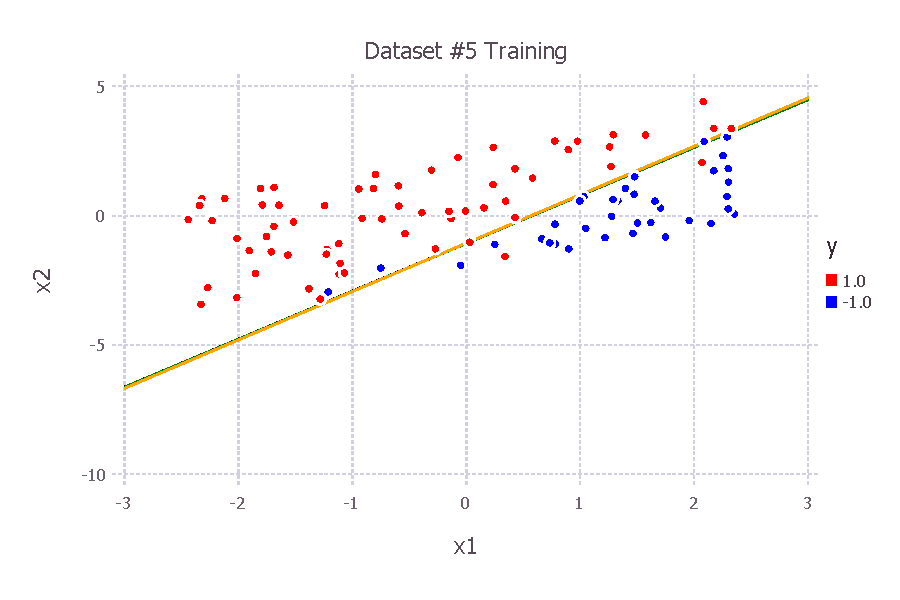
\includegraphics[scale=0.6]{figures/train_final_5.pdf}
    \end{subfigure}
    \quad
    \begin{subfigure}[b]{0.45\textwidth}
	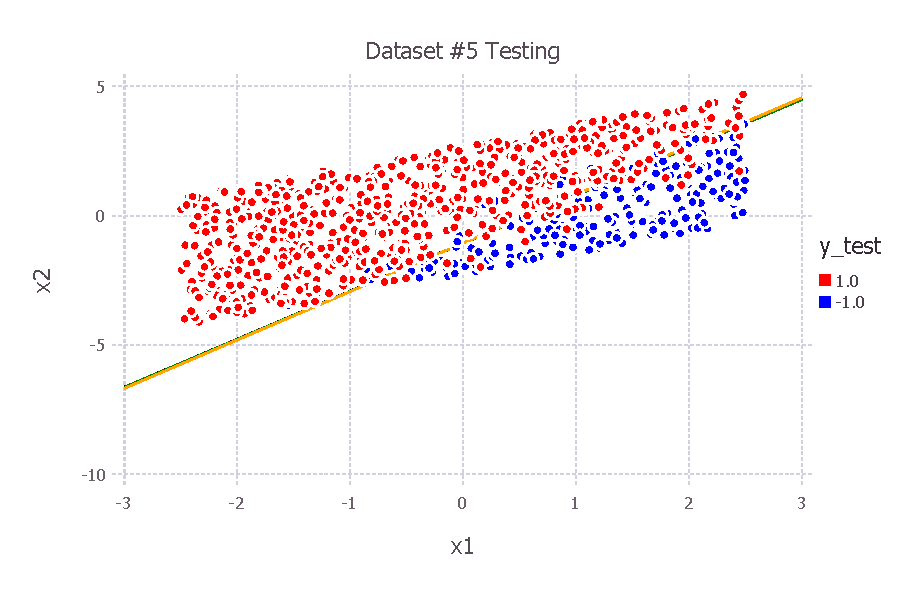
\includegraphics[scale=0.6]{figures/test_final_5.pdf}
	\end{subfigure}
    \caption{Plots of decision boundaries from Dataset 5.}  \label{fig:dataset_5}  
\end{figure}
\begin{figure}[h!]
\centering
    \begin{subfigure}[b]{0.45\textwidth}
	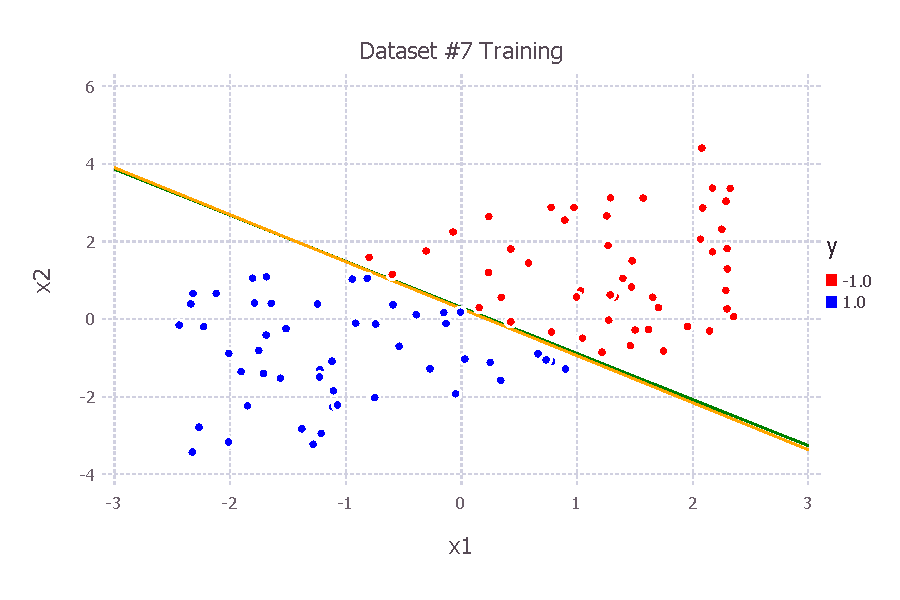
\includegraphics[scale=0.6]{figures/train_final_7.pdf}
    \end{subfigure}
    \quad
    \begin{subfigure}[b]{0.45\textwidth}
	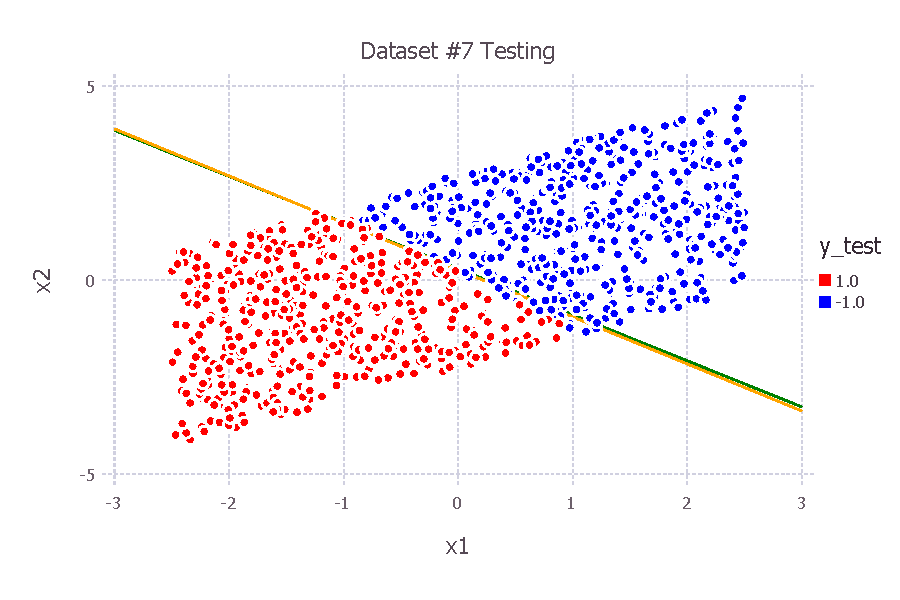
\includegraphics[scale=0.6]{figures/test_final_7.pdf}
	\end{subfigure}
    \caption{Plots of decision boundaries from Dataset 7.}  \label{fig:dataset_7}  
\end{figure}
\begin{figure}[h!]
\centering
    \begin{subfigure}[b]{0.45\textwidth}
	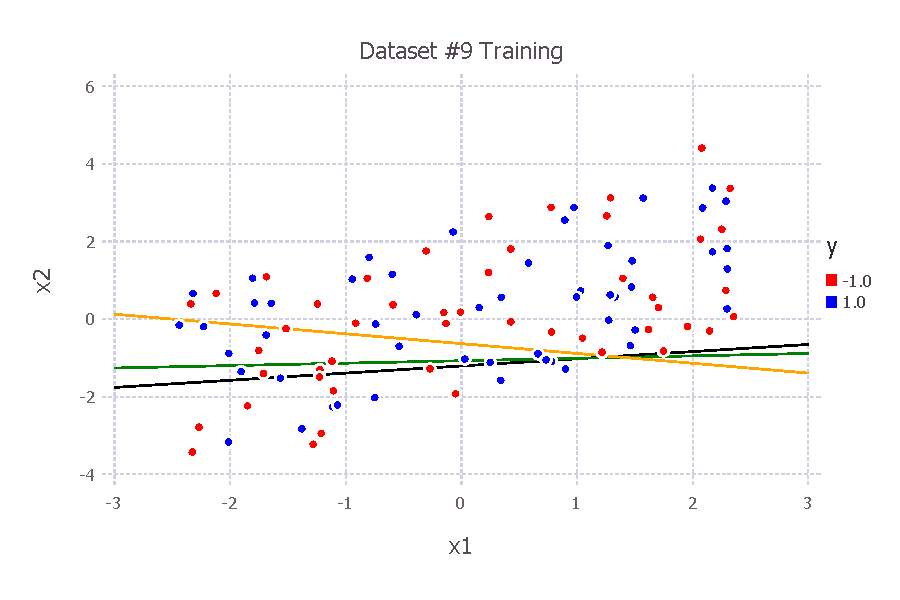
\includegraphics[scale=0.6]{figures/train_final_9.pdf}
    \end{subfigure}
    \quad
    \begin{subfigure}[b]{0.45\textwidth}
	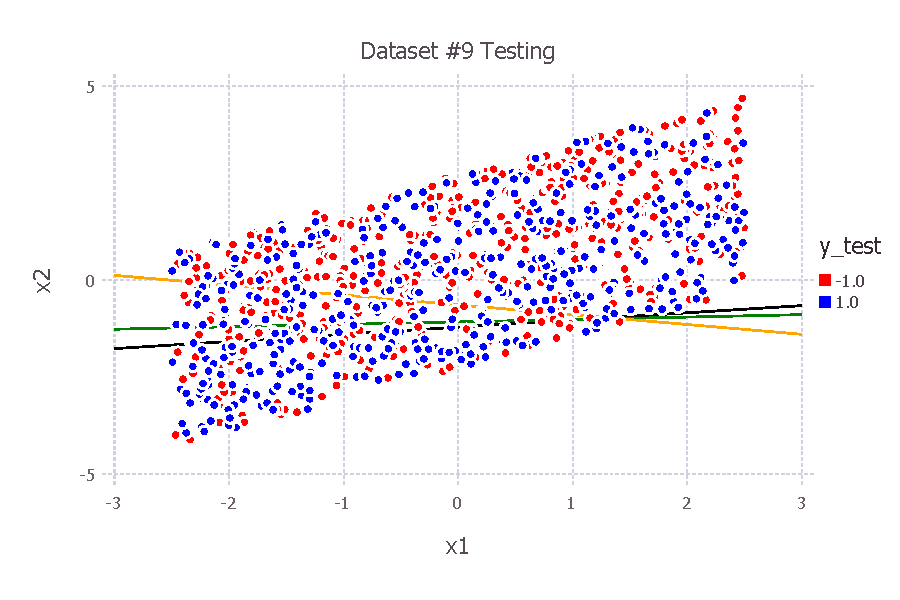
\includegraphics[scale=0.6]{figures/test_final_9.pdf}
	\end{subfigure}
    \caption{Plots of decision boundaries from Dataset 9.}  \label{fig:dataset_9}  
\end{figure}